\section{Problem statement}
\subsection{Road Congestions}
After Munich, Berlin is the city with the most traffic jams in Germany. Peak hour traffic jams are mostly caused by the commuting people. According TomTom \cite{tomtom} data commuting people need to add 12 minutes per 30 minutes in the morning and 16 minutes per 30 minutes in the evening. As a normal employee works around 48 weeks per year and 5 days per week this results in an average time lost of 48 hours in the morning 64 hours in the evening per 30 minutes additional travelling time per year. At figure \ref{averageCongestion} the average percentages of the weekly congestion per hour are visible.

\begin{figure}[h!]
	\centering
	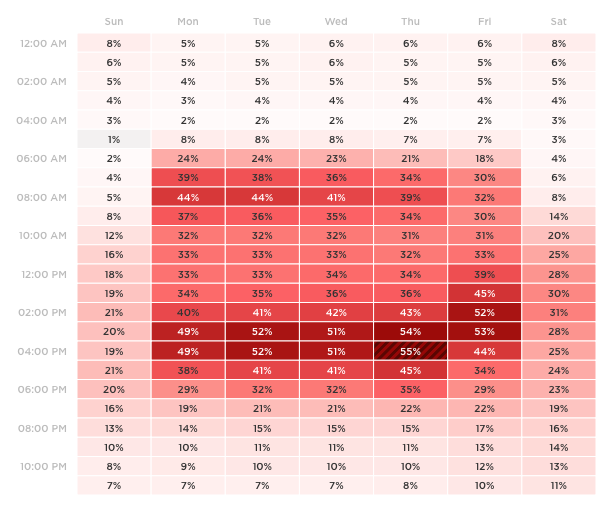
\includegraphics[width=0.55\textheight]{ProblemsFigures/TOMTOMWeeklyAverageCongestion}
	\label{averageCongestion}
	\caption{The average percentage of weekly congestion per hour in Berlin }
\end{figure}

\subsection{Train Delay}
A second big problem for commuting people is train delay. Typically the commuters use  the S-Bahn train \ref{sebsec:sBahn} to enter the city and the fast ICE train if they live at a greater distance of Berlin. As Jens-Peter Schulz, CEO of Dresdner Real Estate Investment Holding \& Chairman told in an article for expo real: 'Germany travellers cheer if their train arrives less than 10 minutes late'. Because the majority of the commuting people live near Berlin we will only analyse the S-Bahn train. People mostly complain that the complete railway system in Germany is not very flexible, once a train has a delay it starts a series of events that causes a lot of delays for other trains as well. Especially when the train becomes very crowded, when this happens the stop time of the trains increases every time. As that train arrives in a transfer station with a delay the other trains wait on that train so it's possible for the passengers to transfer, this results in more trains with a delay. 

\subsection{Ticket price}
The ticket prices for public transport in Berlin are the 5th most expensive of the whole world, this is visibly at figure \ref{pricePT}. As a single ticket costs around 3.16 € and majority of the commuting people need to cover on average 14.3 Km (figure \ref{averageComDis}) to go working. With an average fuel consumption of 4.1 L/100Km (2020) and a fuel price of  1,65 €/L (2021) this means going to work with the car cost around 1 € (parking payment not included). So for people that own a car and do have a parking spot near their work it financially seems to be more attractive to take the car . 

\begin{figure}[h!]
	\centering
	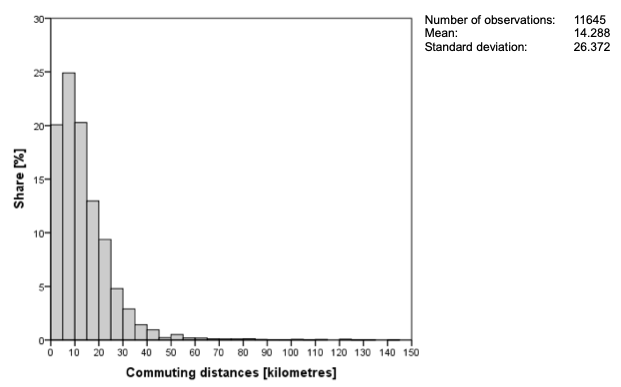
\includegraphics[width=0.55\textheight]{ProblemsFigures/averageCommutingDistance}
	\label{averageComDis}
	\caption{The average distance the commuting people cover. }
\end{figure}

\section{Upcoming changes}


\section{Proposals}